\chapter{Background}
\label{chap:background}

\epigraph{Science is the outcome of being prepared to live without certainty and therefore a mark of maturity. It embraces doubt and loose ends.}{\textit{A.C. Grayling}}

In this chapter, we introduce the main background on the content of this thesis. It covers background on the desiderata, models, and metrics for uncertainty estimation in Machine Learning. In order to preserve the original storyline of the original publications, we kept the background sections in \cref{chap:classification,chap:regression,chap:robustness,chap:graph_data,chap:sequential_data,chap:reinforcement_learning}. Beyond this chapter, we also recommend existing surveys on uncertainty estimation for further details on uncertainty estimation in deep learning \citep{uncertainty-survey,review-uncertainty-dl,psaros2023uncertainty,conformal-survey,hullermeier2021aleatoric}.

\section{Uncertainty desiderata}
\label{sec:background-desiderata}

In this section, we review important desiderata for uncertainty estimation. We provide a summary of these desiderata in \cref{tab:overview_desiderata}.

\begin{table*}[ht]
    \begin{center}
    \resizebox{1.\textwidth}{!}{%
    \begin{tabular}{c}
    \toprule
    \textbf{Bayesian distributions} \\
    \midrule
    \midrule
    $\prior(\bm{\phi} \condition \data)$ where $\bm{\phi}$ are model weights \\
    $\prior(\bm{a} \condition \data, \x)$ where $\bm{a}$ are values of the activations \\
    $\prior(\bm{\theta} \condition \data, \x)$ where $\bm{\theta}$ are parameters of the target distribution \\
    \bottomrule
    \end{tabular}%
    \quad
    \begin{tabular}{c}
        \toprule
        \textbf{Uncertainty types} \\
        \midrule
        \midrule
        Aleatoric uncertainty \\
        Epistemic uncertainty \\
        Predictive uncertainty \\
        \bottomrule
    \end{tabular}%
    \quad
    \begin{tabular}{c}
        \toprule
        \textbf{Practical requirements} \\
        \midrule
        \midrule
        Efficiency: Data \& Time \\
        Flexibility: Architecture \& Optimization \\
        Robustness: Natural \& Adversarial \\
        \bottomrule
    \end{tabular}%
    }
    \end{center}
    \caption{Overview of desiderata for models for uncertainty estimation. Important desiderata involve modelling Bayesian distributions, distinguishing between uncertainty types, and fulfilling practical requirements.}
    \label{tab:overview_desiderata}
\end{table*}

% \begin{table*}[ht]
%     \begin{center}
%     \resizebox{1.\textwidth}{!}{%
%     \begin{tabular}{ccc}
%     \toprule
%     \textbf{Bayesian distributions} & \textbf{Uncertainty types} & \textbf{Practical requirements} \\
%     \midrule
%     \midrule
%     $\prior(\bm{\phi} \condition \data)$ where $\bm{\phi}$ are model weights &  Aleatoric uncertainty & Efficiency: Data \& Time \\
%     $\prior(\bm{a} \condition \data, \x)$ where $\bm{a}$ are values of the activations &  Epistemic uncertainty & Flexibility: Architecture \& Optimization \\
%     $\prior(\bm{\theta} \condition \data, \x)$ where $\bm{\theta}$ are parameters of the target distribution &  Predictive uncertainty & Robustness: Natural \& Adversarial \\
%     \bottomrule
%     \end{tabular}%
%     }
%     \end{center}
%     \caption{Overview of desiderata for models for uncertainty estimation. Important desiderata involve modelling Bayesian distributions, distinguishing between uncertainty types, and fulfilling practical requirements.}
%     \label{tab:overview_desiderata}
% \end{table*}

\subsection{Bayesian Distributions} 

Bayesian distributions offer a convenient framework to express beliefs in the realization of an event. In particular, the Bayesian framework allows to easily incorporate prior knowledge and update our beliefs given additional new observations in a principled way. Hence, we first recall the key concept of the Bayesian framework since it is a core concept in many uncertainty estimation approaches.

\paragraph{Unsupervised learning.} We define the distribution $\prob(\y \condition \bm{\theta})$ over the target variable $\y \in \real^K$ given the parameter $\bm{\theta}$.
Given a dataset $\data=\{\y^{(1)}, ..., \y^{(\ndata)}\}$, the Bayes formula is:
\begin{equation}
    \prior(\bm{\theta} \condition \data) = \frac{\prob(\data \condition \bm{\theta}) \times \prior(\bm{\theta})}{\prob(\data)}
\end{equation}
where $\prob(\data \condition \bm{\theta})$ is the \emph{likelihood}, $\prior(\bm{\theta})$ is the \emph{prior}, $\prior(\bm{\theta} \condition \data)$ is the \emph{posterior}, and $\prob(\data)$ is the \emph{evidence}.
Intuitively, the Bayesian formula updates the prior belief represented by $\prior(\bm{\theta})$ into the posterior belief represented by $\prior(\bm{\theta} \condition \data)$ after observing a dataset $\data$ \cite{bishop}.
The choice of prior is crucial. A common choice is to follow the \emph{principle of maximum entropy} \citep{maximum-entropy-principle} and enforce high entropy for the prior distribution which is usually considered less informative. However, note that many works studied different choices of priors \cite{jeffreys1946prior, silvestro2020prior}.
The evidence term $\prob(\data)$ corresponds to a normalization constant which can sometimes be ignored \cite{bishop}.

After observing a dataset $\data$, we can update the distribution over the target variable $\y$ in two ways.
A first option is to use a point-wise estimate of the target distribution parameter, i.e.:
\begin{equation}
    \prob(\y \condition \bm{\theta}^*)
\end{equation}
where $\bm{\theta}^*=\argmax\prior(\y \condition \bm{\theta})$ would be the maximum likelihood estimate, or $\bm{\theta}^*=\argmax\prior(\bm{\theta} \condition \data)$ would be the maximum a posteriori estimate.
A second option is to integrate over all possible values for the target distribution parameter, i.e.:
\begin{equation}
    \label{eq:posterior_predictive}
    \prob(\y \condition \data) = \int \prob(\y \condition \bm{\theta}) \prior(\bm{\theta} \condition \data) d\bm{\theta}
\end{equation}
where $\prob(\y \condition \data)$ is called the posterior predictive distribution. 
This second approach is often considered to be more Bayesian since it depends on the full posterior distribution $\prior(\bm{\theta} \condition \data)$.
However, it might be costly to compute the posterior distribution since it requires integration.

\paragraph{Supervised learning.} In supervised learning, the goal is to predict the value of a target output variable $\y$ given an input $\x$ after observing a dataset $\data=\{(\x^{(1)}, \y^{(1)}), ...,$ $(\x^{(\ndata)}, \y^{(\ndata)})\}$.
In this case the posterior predictive requires to be adapted with three main options: compute the posterior distribution over the weights $\prior(\bm{\phi} \condition \data)$, compute the posterior over the activations $\prior(\bm{a} \condition \data, \x)$, and compute the posterior over the parameters of the target distribution $\prior(\bm{\theta} \condition \data, \x)$ (see \cref{tab:overview_desiderata} left). The first option is:
\begin{equation}
    \label{eq:factorization_1}
    \prob(\y \condition \data, \x) = \int \prob(\y \condition \bm{\phi}, \x) \prior(\bm{\phi} \condition \data) d\bm{\phi}
\end{equation}
where $\bm{\phi}$ denote the model weights. In this case, the parameter distribution $\prior(\bm{\phi} \condition \data)$ is not conditioned on the input $\x$ and only accounts for an uncertainty dependent on the dataset $\data$. Examples of such models are Bayesian neural networks which learn Bayesian distribution $\prior(\bm{\phi} \condition \data)$ where $\bm{\phi}$ denote the model weights \cite{bayesian-networks}.
The second option is:
\begin{equation}
    \label{eq:factorization_2}
    \prob(\y \condition \data, \x) = \int \prob(\y \condition \bm{a}) \prior(\bm{a} \condition \data, \x) d\bm{a}
\end{equation}
where $\bm{a}$ denote intermediate representations of $\x$. In this case, the parameter distribution $\prior(\bm{a} \condition \data, \x)$ is conditioned on the new input $\x$ and accounts for an uncertainty dependent on the input $\x$. Examples of such models are Bayesian neural networks which learn Bayesian distribution $\prior(\bm{a} \condition \data, \x)$ where $\bm{a}$ denote the values of the activations \cite{gp-uncertainty-activation,natural-parameter-network}.
Alternatively, the third option is:
\begin{equation}
    \label{eq:factorization_3}
    \prob(\y \condition \data, \x) = \int \prob(\y \condition \bm{\theta}) \prior(\bm{\theta} \condition \data, \x) d\bm{\theta}
\end{equation}
where $\bm{\theta}$ denote the direct parameters of the distribution over the target $\y$. In this case, the parameter distribution $\prior(\bm{\theta} \condition \data, \x)$ is conditioned on the new input $\x$ and also accounts for an uncertainty dependent on the input $\x$. Examples of such models are the Bayesian neural networks proposed in this thesis \cite{charpentier2020,natpn, graph-postnet,charpentier2022uncertainty-rl,uceloss} which learn Bayesian distributions $\prior(\bm{\theta} \condition \data, \x)$ where $\bm{\theta}$ denote the parameters of the distribution over the target labels $\y$. In this thesis, we focus on learning  Bayesian distributions on the (generally) low dimensional target parameters $\bm{\theta}$, in contrast to the (generally) high dimensional activation $\bm{a}$ or weights  $\bm{\phi}$, thus advantageously allowing to reduce the computation complexity of the posterior distribution.

\subsection{Aleatoric, Epistemic \& Predictive Uncertainty}

The Bayesian formula in \cref{eq:posterior_predictive} involves three types of distribution (i.e. $\prob(\y \condition \bm{\theta})$, $\prior(\bm{\theta} \condition \data)$, and $\prob(\y \condition \data)$) which cover the three main sources of uncertainty introduced below: the aleatoric uncertainty represented by the distribution $\prob(\y \condition \bm{\theta})$, the epistemic uncertainty represented by the distribution $\prior(\bm{\theta} \condition \data)$, and the predictive uncertainty represented by the distribution $\prob(\y \condition \data)$ (see \cref{tab:overview_desiderata} middle).
In practice, each uncertainty type can be measured by computing the spread of its respective distribution with the (differential) entropy which represents its variability, i.e. \citep{PriorNetworks,uncertainty-deep-learning}:
\begin{align}
     u_\text{alea} = \entropy[\prob(\y \condition \bm{\theta})], \hspace{4mm}
     u_\text{epist} = \entropy[\prior(\bm{\theta} \condition \data)], \hspace{4mm}
     u_\text{pred} = \entropy[\prob(\y \condition \data)]
\end{align}
Apart from the entropy, other uncertainty metrics commonly use the variance of the distributions to indicate their variability. Finally, it is also to measure the variability of a distribution with their concentration parameters if they exist.

\textbf{Aleatoric uncertainty.} The \emph{aleatoric uncertainty} is sometimes also called data uncertainty, stochastic uncertainty or risk \cite{hullermeier2021aleatoric,knight1921, malini2018}. 
The aleatoric uncertainty is represented by the distribution $\prob(\y \condition \bm{\theta})$.
Beyond entropy computation, it can also be computed using max probability for classification \cite{malini2018}.
The aleatoric uncertainty should be high when \emph{the model does not know because of inherent noise in a given context} (e.g. noisy environment, noisy sensors, low computation resources, model mispecification) \cite{wenger2022posterior, hullermeier2021aleatoric}.
Given a specific context, the aleatoric uncertainty is \emph{irreducible} since additional observations cannot resolve the information loss due noisy measurements or misspecifications. 
However, aleatoric uncertainty can be reduced by using higher measurement resolution or improving the model specification. 

\textbf{Epistemic uncertainty.} The \emph{epistemic uncertainty} is sometimes also called knowledge uncertainty, systematic uncertainty, or knightian uncertainty \cite{hullermeier2021aleatoric,knight1921,malini2018}.
The epistemic uncertainty is represented by the distribution $\prior(\bm{\theta} \condition \data)$.
The epistemic uncertainty should be high when \emph{the model does not know because of a lack of observed data} in the dataset $\data$.
Hence, the epistemic uncertainty is \emph{reducible} since it should decrease when collecting additional data.

\textbf{Predictive uncertainty.} The \emph{predictive uncertainty} is sometimes also called total uncertainty \cite{hullermeier2021aleatoric,malini2018}.
The predictive uncertainty is represented by the distribution $\prob(\y \condition \data)$.
Intuitively, the predictive uncertainty aggregates the effect of the aleatoric and epistemic uncertainty by integrating jointly the distributions $\prob(\y \condition \bm{\theta})$ and $\prior(\bm{\theta} \condition \data)$. 

In this thesis, we focus on methods capable to estimates the three types of uncertainty types.

\subsection{Efficiency, Flexibility \& Robustness}

Uncertainty methods are also expected to have practical characteristics (see \cref{tab:overview_desiderata} right). 

First, an uncertainty method is expected to be \emph{efficient} at both training and testing time. 
A first aspect is \emph{time efficiency} meaning that the method should be fast with low computational overhead. E.g. uncertainty methods requiring multiple forward passes are usually more expensive than method require a single forward pass.
As second aspect is \emph{data efficiency} meaning that the method should require as few data as possible to train.

Second, an uncertainty method is expected to be \emph{flexible}.
A first aspect is \emph{architecture flexibility} meaning that the method should easily adapt to any architectures in order to easily adapt to different input types (e.g. tabular, images, graphs, and sequential data) and output types (e.g. classification and regression).
A second aspect is \emph{optimization flexibility} meaning that the method should easily adapt to different training schemes including end-to-end training or fine-tuning based on pretrained models.

Finally, an uncertainty method is expected to be \emph{robust}.
A first aspect is \emph{natural robustness} meaning that the method should be performant even if there is some natural drift in the data. Natural drifts could be due to time evolution or location variability \cite{wilds, neuhold201mapillary, shifts-dataset}.
A second aspect is \emph{adversarial robustness} meaning that the method should be performant even against adversarial perturbations which are specifically designed to fool the model. Adversarial perturbations can be viewed as the worst-case scenario for the model. Different methods to compute adversarial perturbations including white box attacks which do not have information about the model, black box attacks which have full access to the model information, and gray box which have partial information about the model \cite{han2020adversarial}.

In this thesis, we focus on proposing practical methods which are efficient in terms of data and time, flexible in terms of architecture and optimization schemes, and robust in terms of natural and adversarial perturbations.

\section{Uncertainty models}
\label{sec:background-models}

In this section, we review important families of models for uncertainty estimation. We provide a summary of these models in \cref{fig:overview_methods}. We refer the reader to seed papers and surveys provided in the following paragraphs presenting each family of methods for a detailed presentation of their concepts. Overall, we observed that these families of methods could be approximately be classified in two groups. On one hand, ensembles, Monte Carlo dropout, Markov chain Monte Carlo, variational inference, Laplace approximation, and Gaussian process methods form a first group of methods with strong Bayesian guarantees but often requiring expensive computations. On the other hand, evidential, calibration, density-based, energy-based, and distance-based methods form a second group of methods sometimes capable of efficient uncertainty predictions to the cost of weaker Bayesian guarantees or additional practical constraints like the need of additional training or validation data.

\begin{figure}[ht!]
    \centering
    \begin{subfigure}[t]{1. \columnwidth}
        \centering
        $\vcenter{\hbox{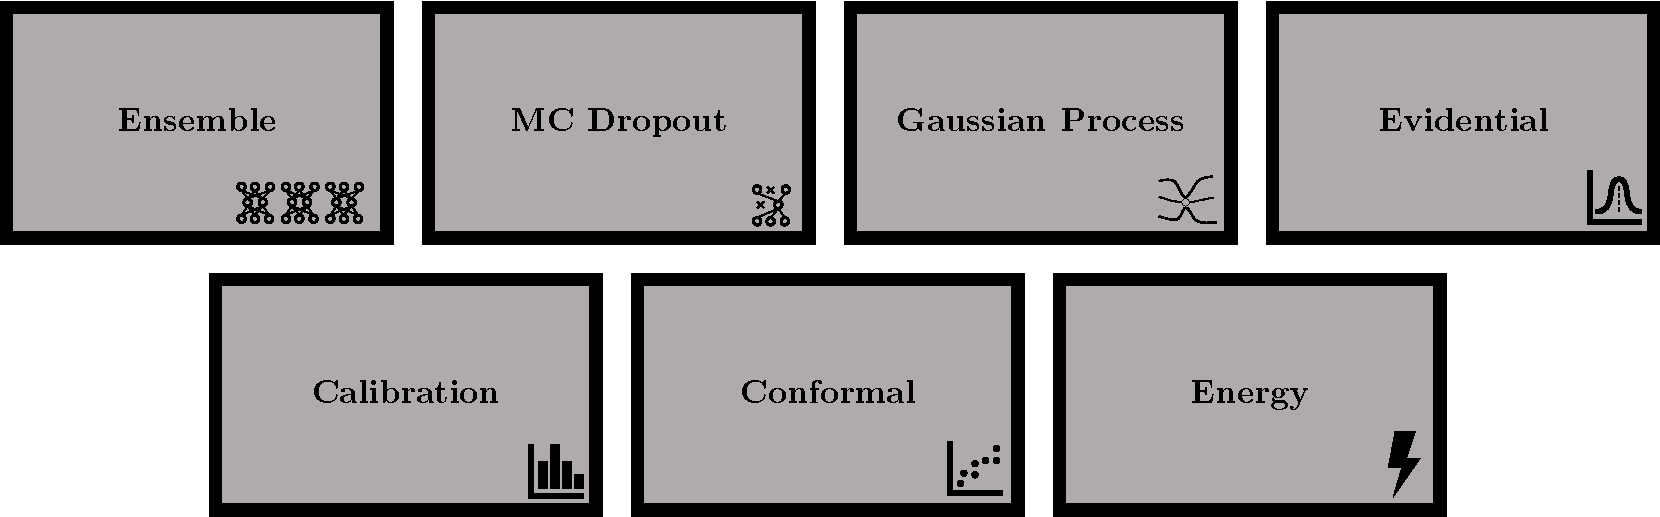
\includegraphics[width=0.9 \textwidth]{resources/overview_methods.pdf}}}$
    \end{subfigure}%
    \caption{Overview of the different families of methods for uncertainty estimation.}
    \label{fig:overview_methods}
	% \vspace{-.5cm}
\end{figure}

% Add a table with useful existing implementations/packages of those methods

\paragraph*{Ensembles.} This family of methods consists in combining the predictions of a set of multiple models $f_{\bm{\phi}_1},\cdot, f_{\bm{\phi}_K}$ by using stacking, bagging, boosting, Bayesian averaging or other Bayesian combinations \citep{bayesian-averaging-to-combination}. The variance of the different model predictions can be viewed as uncertainty estimates. These uncertainty estimates can be considered Bayesian where the member weights are sampled from the posterior weight distribution, i.e. $\bm{\phi}_k \sim \prior(\bm{\phi} \condition \data)$. The ensembles can be \emph{homogeneous ensembles}, i.e. the models share the same architecture, be \emph{heterogeneous ensembles}, i.e. the models have different architectures, or \emph{implicit ensembles}, i.e. a single model approximated ensembles parameter sampling \citep{abe2022deep}. Further, the different models can be trained sequentially (see e.g. \citep{schapire2013explaining, chenG16xgboost}) or independently (see e.g. \citep{ensembles}).
%
Ensembles are considered as strong baselines in terms of uncertainty estimation and predictive performances \citep{dataset-shift}. Ensembles also benefit from a simple implementation \citep{ensembles}.
%
Ensembles are often considered to be expensive as they require multiple forward passes. Many approaches \citep{batch-ensembles,mimo-independent-subnetworks} proposed to make faster ensembles. Further, while ensembles improve predictive performance, this performance gain can actually be replicated through the use of (larger) single models \citep{abe2022deep}.

\paragraph*{Variational Inference.} This family of methods consists in approximating a (generally intractable) posterior distribution with a variational distribution belonging to a tractable family of distributions \cite{blei2017vi}. The approximate posterior distribution is often optimized using an Evidence Lower Bound (ELBO) loss. Many methods (see e.g. \cite{practical-bnn,bayesian-networks,practical_deep_bayesian_principles}) are interested in the posterior distribution over the model weights, i.e. $\prior(\bm{\phi} \condition \data)$ where $\bm{\phi}$ are the model weights. Thus, similarly to ensembles, uncertainty estimates can be obtained by sampling from the posterior distribution on the weights and computing the variance of their predictions. These methods generally needs to trade off the expressivity of the posterior distribution with computational complexity. To approximate the posterior distribution over the high dimensional weights, many works proposed to use techniques like mean-field approximations \citep{practical-bnn,bayesian-networks,practical_deep_bayesian_principles}, normalizing flows \cite{radialflow,Louizos2017}, or matrix decomposition with low rank or Kronecker products \cite{mishkin2018slang,bae2018eigen,zhang2017noisy}. In contrast with methods which are interested in posterior distributions $\prior(\bm{\phi} \condition \data)$ over model weights $\bm{\phi}$, we present in this thesis variational methods which approximate the posterior distribution $\prior(\bm{\theta} \condition \data, \x)$ over the target distribution parameters $\bm{\theta}$ (see \cref{chap:classification,chap:regression}).

\paragraph*{Monte Carlo Dropout.} Monte Carlo (MC) dropout consists in randomly dropping neurons to form different models $f_{\bm{\phi}_1},\cdot, f_{\bm{\phi}_K}$ and combine their predictions \citep{dropout} at both training and testing time. This approach can be considered as an ensemble of implicit models \citep{abe2022deep} but also as performing variational inference \citep{dropout}. Hence, similarly to ensembles, the variance of the predictions can be viewed as Bayesian uncertainty estimates the member weights are sampled from the posterior weight distribution, i.e. $\bm{\phi}_k \sim \prior(\bm{\phi} \condition \data)$. Many works extended this approach for e.g. convolutional layers \citep{tassi2020bayesian} or dropping connection instead of activations \citep{wan2013dropconnect}.

\paragraph*{Markov Chain Monte Carlo.} Markov Chain Monte Carlo (MCMC) methods, consists in building a Markov Chain which will converge to samples from the posterior distribution. A key example is the Metropolis-Hastings algorithm which iteratively draw a sample from a transition rule and then decide to accept or reject it \cite{robert2015metropolis}. Many works focus on sampling from the approximate posterior distribution $\prior(\bm{\phi} \condition \data)$ over model weights $\bm{\phi}$ (see e.g. \citep{duane1987hybrid,welling2011langevin}). In this case, the Markov Chain builds a sequence $\bm{\phi},\cdot,\bm{\phi}_t$ by following e.g. Hamiltonian dynamics \citep{duane1987hybrid} or Stochastic Gradient Langevin Dynamics \cite{welling2011langevin,garriga-alonso2021exact,ma2015mcmc} which converge to sample from the posterior distribution, i.e. $\bm{\phi}_t \sim \prior(\bm{\phi} \condition \data)$ when $t \rightarrow \infty$. On one hand, while full batch MCMC has managed to scale to modern tasks and models, they often come at a heavy computational cost \citep{what-bnn-posterior}. On the other hand, while stochastic gradient MCMC improve the computational efficiency \cite{welling2011langevin,garriga-alonso2021exact,ma2015mcmc}, it might introduce bias in the stationary distribution by omitting the Metropolis-Hasting rejection or subsampling the data \citep{betancourt2015data,what-bnn-posterior}.

\paragraph*{Laplace Approximation.} The Laplace approximation consists in approximating the posterior distribution with a Gaussian distribution centered around a mode of the posterior distribution. Many works focus on approximating the posterior distribution $\prior(\bm{\phi} \condition \data)$ over model weights $\bm{\phi}$. In this case the Laplace approximation gives:
\begin{align*}
    \prior(\bm{\phi} \condition \data) \approx \DNormal(\bm{\phi}_\text{MAP}, \bm{\Sigma})
\end{align*}
where $\bm{\phi}_\text{MAP}$ is the maximum a posteriori estimate, and $\bm{\Sigma}=-(\nabla_{\bm{\phi}}^2 \left.\loss(\data;\bm{\phi})\right|_{\bm{\phi}_\text{MAP}})^{-1}$ is the Laplace approximation of the covariance based on the Hessian of the loss. The posterior distribution can be defined on all model weights, subnetworks \cite{daxberger2021bayesian}, or only the last layer \cite{bayesian-a-bit}. The Hessian computation can be costly and can be approximated using the different techniques like the Fisher information matrix, the generalized Gauss-Newton matrix, diagonal factorization, Kronecker-factored approximate curvature, or low-rank approximation \citep{daxberger2021laplace}. Finally, the computation of the predictive distribution needs further approximation like linearizing the neural network or using Monte-Carlo approximation \citep{daxberger2021laplace}.

\paragraph*{Gaussian Process.} Gaussian Processes (GPs) are a family of Bayesian methods which, given a dataset $\data$, associates to each new input $\x$ a predictive Gaussian distribution over the output $\y \sim \prob(\y \condition \data, \x) = \DNormal(m(\x), \sigma^2(\x))$. The mean function $m(\x)$ and the variance function $\sigma^2(\x)$ depends on the kernel function $\kappa(.,.)$ which encodes the similarity between data samples. Intuitively, uncertainty estimates can be obtained by computing the variance or the entropy of the predicted Gaussian distribution.
On one hand, standard GPs have computational and storage limitations \cite{jakkala2021deepgp}. E.g. the computation of the variance function is cubic in the number of data samples which does not scale well to large datasets. To mitigate this issue, previous works proposed sparse Gaussian process which introduce variational pseudo-points can be optimized with stochastic gradient descent (see e.g. \cite{snelson2005sparse,titsias2010gplvm,due}).
On the other hand, standard GPs does not naturally extract hierarchical representations from structured data. To mitigate this issue, previous works proposed e.g. to use multilayer GPs \cite{damianou2012deepgp} or deep neural networks as the kernel function \cite{wilson2016stochastic}. We refer to existing survey on Gaussian process in deep learning for further details \citep{gp-for-ml,damianou2012deepgp,jakkala2021deepgp}.

\paragraph*{Evidential.} Evidential methods are derived from the theory of evidence which can be seen as generalization of the Bayesian theory to subjective probables \cite{dempster1968evidence,shafer1976mathematical}. Instead of predicting directly the parameters $\bm{\theta}$ of the target distribution $\prob(\y \condition \bm{\theta})$, evidential methods consist in predicting the parameters of the distribution $\prior(\bm{\theta} \condition \data, \x)$ defined over the parameters $\bm{\theta}$, thus following the factorization in \cref{eq:factorization_3}. In this case, uncertainty estimates can be obtained by computing the variance or the entropy of the predicted target or evidential distributions. This family of models is generally effective since it only requires a single forward pass for uncertainty estimation. To improve performances of evidential models, other works proposed to use OOD data during training \cite{PriorNetworks,reverse-kl}, knowledge distillation \cite{distribution-distillation}, or contrastive learning \cite{uncertainty-generative-classifier}. In this thesis, we introduce a new family of evidential models called \emph{Posterior networks} with a clear Bayesian interpretation and low practical overhead (see \cref{chap:classification,chap:regression,chap:robustness,chap:graph_data,chap:sequential_data,chap:reinforcement_learning}). We refer to existing survey on evidential deep learning for uncertainty quantification for further details \citep{survey_evidential_uncertainty}.

\paragraph*{Calibration.} Calibration metrics consists at evaluating if the probabilities predicted by a model correspond to the true probabilities of the model to be correct (see \cref{sec:calibration} for further details). Hence, in order to achieve high performance w.r.t. calibration metrics, calibration methods aim at predicting probabilities which are good approximations of their true probability of correctness. Beyond uncertainty-aware models which are expected to be well-calibrated, we distinguish between two other groups of calibration methods: during-training calibration methods and post-training calibration methods. During-training calibration methods apply regularization techniques in the loss objective to create inherently calibrated models (see e.g. \cite{lee2018training,corbieres2019confidence,minderer2021revisiting}). Post-training calibration methods recalibrate the model predictions after training (see e.g. \cite{calibration-network,wenger201calibration}). While these methods can adapt well to different architectures types, they usually require additional held-out validation data and assume that validation and test distribution are similar. Prominent classes of post-training calibration method are histogram binning \cite{zadrozny2001calibrated}, Temperature scaling \cite{calibration-network}, isotonic calibration \cite{zadrozny2002transforming}, Dirichlet calibration \cite{kull2019beyond}, or conformal predictions \cite{conformal-survey,marx2022conformal}.

\paragraph*{Density-based models.} This family of models assigned to every data sample $\x$ a probability density estimate $\prob(\x \condition \bm{\phi})$. In this case, a data sample considered uncertain by the model should be assigned a low density value while a data sample considered certain for the model should be assigned a high density value. The density estimator can be of different nature like a mixture of Gaussian \cite{simple_ood_adv_detection,du2022vos} or a normalizing flow \cite{nf-review,why-nf-fail-ood,postels2020hiddenuncertainty}. The choice of space on which the density estimator operates is crucial. While density estimation on the input space might be difficult due to the curse of dimensionality \citep{anomaly-detection,deep-generative,typicality_OOD_generative}, other works \cite{charpentier2020, why-nf-fail-ood, density-states-ood, contrastive-ood} improved the performance of density-based methods on uncertainty tasks by leveraging a task-induced bias or low-dimensional statistics. In particular, density-based models methods have achieved impressive success in OOD detection tasks \cite{ood-detection-survey}.

\paragraph*{Energy-based models.} Energy-based models (EBMs) associate to every combination of input $\x$ and output $\y$, a scalar energy value $E_{\bm{\phi}}(\y, \x)$ \cite{lecun2006tutorial}. Interestingly, EBMs can often be viewed as density-based models. Indeed, the energy function $E_{\bm{\phi}}(\y, \x)$ can be transformed into Gibbs distributions $\prob(\y \condition \bm{\phi}, \x)$, $\prob(\y, \x \condition \bm{\phi})$, or even $\prob(\x \condition \bm{\phi})$ given some integrations constraints on $E_{\bm{\phi}}(\y, \x)$, thus assigning uncertainty estimates on for different combinations of variables $\y, \x$ \cite{energy_based_classifier}. In this case, low predicted energy values correspond to high uncertainty estimates. EBMs are flexible models capable to achieve great performances in OOD detection in many tasks \citep{energy-ood,wang2021ebm} as long as they can capture semantic features of the data \cite{ood_ebm}.

\paragraph*{Distance-based models.} The core idea of distance-based methods is that the model should assign high uncertainty to testing data samples which are far away from training data samples. Hence, distance-based models can e.g. use distance to class centroids \cite{mohseni2020self}, nearest-neighbor \cite{sun2022knnood}, or inducing points \cite{due} to estimate uncertainty. Further, they can also use Mahalanobis distance \cite{mohseni2020self}, euclidean distance \cite{huang2021feature}, or geodesic distance \cite{gomes2022igeood}. Similarly to density-based models, distance-based models can also achieve great performance in OOD detection tasks \cite{ood-detection-survey}. Further, distance awareness has been shown to be an important component for uncertainty estimation tasks \cite{uncertainty-distance-awareness,due}.

% \subsection{Sampling-based models}
% Sampling-based models estimate uncertainty by aggregating statistics (e.g. mean and variance) from different samples from a given distribution. The prediction generally follows a three steps process:
% \textbf{(1)} we sample $K$ model weights $\bm{\phi}_k$ from a distribution over the weights $\prior(\bm{\phi} \condition \data)$, i.e. $\bm{\phi}_k \sim \prior(\bm{\phi} \condition \data)$. The type of the weight distribution $\prior(\bm{\phi} \condition \data)$ is a key design choice. E.g. ensemble proposes to train independent model weights \cite{ensembles}, MC dropout randomly drop weights with given dropout rate \cite{dropout}, and other Bayesian neural networks learn explicit distributions like Gaussian over the model weights \cite{bayesian-networks}. \textbf{(2)} We perform $K$ forward passes with the sampled model weights to obtain parameters $\bm{\theta}_k$ of the target distribution, i.e. $\bm{\theta}_k = f_{\bm{\phi}_k}(\x) \text{ for } k=\{1,\cdot,K\}$. This allows to implicitly sample the parameters $\bm{\theta}_k$ from the posterior distribution $\prior(\bm{\theta} \condition \data, \x)$, i.e. $\bm{\theta}_k \sim \prior(\bm{\theta} \condition \data, \x)$. In this case, the parameters $\bm{\theta}_k$ can be the parameters of a categorical distribution for classification or the parameters of a Gaussian distribution for regression. \textbf{(3)} We aggregate the $\bm{\theta}_k$ parameters to form a point estimate $\bm{\theta}*$, e.g. $\bm{\theta}*=\frac{1}{K}\sum_k \bm{\theta}_k$. This allows to define the target distribution $\prob(\y \condition \bm{\theta}^*)$. These methods are flexible and allows to estimate all types of uncertainty while still being accurate. However, they often come to the cost of a higher computational cost due to the need of multiple forward passes.

% \subsection{Sampling-free models}
% Sampling-free models are capable of estimating uncertainty in a single forward pass. A first family of models explicitly parametrize the distribution $\prior(\bm{\theta} \condition \data, \x)$ with evidential distributions \citep{survey_evidential_uncertainty,robustness-uncertainty-dirichlet,max_gap_id_ood,uncertainty-generative-classifier,multifaceted_uncertainty,graph-postnet, lightweight-prob-net}. A second family aims at learning deep Gaussian processes on a learned latent space \citep{uncertainty-distance-awareness, due, duq, uceloss}. A third family aims at learning deep energy-based models \citep{ood_ebm, jem_ebm}. The GP and energy-based approaches might sometimes not be able to disentangle the different uncertainty types. Another family of models tries to recalibrate existing models by using calibration methods like temperature scaling \cite{calibration-network} or conformal predictions \cite{conformal-survey}. Calibration and conformal prediction methods generally require additional data to calibrate uncertainty estimates. Finally, a last family of models propagate uncertainty across layers \citep{natural-parameter-network, sampling-free-variance-propagation, feed-forward-propagation, lightweight-prob-net, probabilistic-backprop-scalable-bnn}. They model uncertainty at the weight and/or activation levels and are generally constrained to specific transformations.

\section{Uncertainty metrics}
\label{sec:background-experiments}

While ML models are primarily expected to provide accurate predictions, we present in this section an exhaustive summary of the main metrics used to evaluate the quality of uncertainty estimation. 
It covers correct/wrong predictions detection, OOD \& dataset shifts detection, calibration, and sample efficiency.
We provide a collection of evaluation setup covering various tasks to benchmark uncertainty models in \cref{tab:overview_evaluation}. Beyond these metrics, note that Bayesian methods have been also used in other tasks like  model pruning, model selection, or hyper-parameter tuning \citep{bayesian-networks,daxberger2021laplace}.

\begin{table*}[ht]
    \begin{center}
    \resizebox{1.\textwidth}{!}{%
    \begin{tabular}{ccc}
    \toprule
    \textbf{Uncertainty metrics} & \textbf{Existing evaluation setups} & \textbf{Practical reason}\\
    \midrule
    \midrule
    Uncertainty calibration & \cite{dataset-shift, chung2021uncertainty,nado2021uncertainty, tran2022plex} & \emph{Fairness}, \emph{Trust}\\
    \midrule
    Correct/wrong pred. detection & \cite{robustness-uncertainty-dirichlet,Hendrycks2016, shifts-dataset, tran2022plex} & \emph{Trust} \\
    \midrule
    OOD detection & \cite{robustness-uncertainty-dirichlet,charpentier2022uncertainty-rl,yang2022openood, cao2020ood, kirchheim2022pytorch, Hendrycks2016,charpentier2022uncertainty-rl, tran2022plex} & \emph{Safety}\\
    \midrule
    Robustness to dataset shifts & \cite{robustness-uncertainty-dirichlet,wilds, neuhold201mapillary, shifts-dataset, benchmarking-corruptions, taori2020shift, dataset-shift, croce2021robustbench,charpentier2022uncertainty-rl, tran2022plex} & \emph{Maintenance} \\
    \midrule
    Sample efficiency & \cite{charpentier2022uncertainty-rl,hsu2018continual, lin2021clear,antoniou2020fewshots,tran2022plex} & \emph{Development, Maintenance}\\
    \bottomrule
    \end{tabular}%
    }
    \end{center}
    \caption{Overview of metrics for uncertainty estimation. We relate each of the uncertainty metric to existing evaluation setups and practical reason for uncertainty estimation presented in \cref{sec:why_uncertainty}}
    \label{tab:overview_evaluation}
\end{table*}

\subsection{Uncertainty Calibration}
\label{sec:calibration}

It is crucial to provide confidence intervals accurately reflecting the true chance of an event to happen. This allows to increase \emph{fairness} and \emph{trust} of the ML prediction even on under-represented data regions. Intuitively, if the model predict $80\%$ chance for a class to be the correct one, we would expect the model to be $80\%$ of the time correct. Hence, uncertainty estimates are important to answer the following practical question:

\begin{center}
    \textbf{Does probabilities predicted by ML models correspond to the true probabilities?}
\end{center}

In practice, the confidence intervals provided by the models can be used to estimate risks when making decisions. Appropriate metrics to evaluate calibration involve (strictly) proper scoring rules like Brier scores for classification and quantiles scores for regression \cite{scoring-rules}.

\subsection{Correct \& Wrong Predictions}

It is also crucial to detect when ML models are likely to provide correct or wrong predictions. This allows to increase \emph{trust} in the model predictions, especially when the predictions are used to make important decisions. Intuitively, while the model predictions should be accurate, uncertainty estimates should also be good indicators of the prediction errors. Indeed, high uncertainty should indicate likely wrong prediction while low uncertainty should indicate likely correct predictions. Hence, uncertainty estimates are important to answer the following practical question:

\begin{center}
    \textbf{Can we detect prediction errors of ML models?}
\end{center}

In practice, each application would require to set a threshold on the uncertainty estimates. Ideally, while predictions associated with uncertainty estimates below this threshold should be correct, the predictions associated with uncertainty estimates above this threshold should be wrong. Hence, we can use evaluation metrics which compare scores (i.e. uncertainty estimates) with binary classes (i.e. correct/wrong predictions). Common metrics are based on false and true positive and negative rates given a specific threshold like precision, recall, or F1 score \cite{powers2011evaluation}. However, these metrics have the important limitation to depend on a specific choice of threshold. Instead, there exist other evaluations like receiving operator curves (ROC) and precision-recall curves (PR) which can compare the prediction correctness and the predicted uncertainty scores for any choice of threshold. In particular, the area under the ROC curve (AUC-ROC) and the area under the PR curve (AUC-PR) are appropriate metrics to evaluate the overall performance of the uncertainty scores independently of the choice of threshold \cite{apr_auroc}. All the data used for the evaluation of the correct/wrong predictions should be relevant to the task meaning that every input has a corresponding output label. This requirement contrasts data used for out-of-distribution detection data where inputs might not have corresponding labels.

\subsection{Out-Of-Distribution}

It is crucial to detect when incoming data are anomalous to increase the \emph{safety} of model predictions. The anomalous data are often considered out-of-distribution (OOD) in contrast with normal data similar to data observed during training which are considered in-distribution (ID). Intuitively, uncertainty estimates should be good indicators of anomalous data. Indeed, high uncertainty should indicate likely abnormal data while low uncertainty should indicate likely normal data. Hence, uncertainty estimates are important to answer the following practical question:

\begin{center}
    \textbf{Can uncertainty estimates detect anomalous data?}
\end{center}

Similarly to the detection of correct and wrong predictions, the detection of anomalous data would also require to set a threshold on the uncertainty estimates. In this case, while predictions associated with uncertainty estimates below this threshold should be normal ID data, predictions associated with uncertainty estimates above this threshold should ideally be abnormal OOD data. Hence, we can also use evaluation metrics like precision, recall, AUC-ROC, and AUC-PR which compare scores (i.e. uncertainty estimates) with binary classes (i.e. ID/OOD data). While ID data should be relevant to the task (i.e. ID inputs have output labels), the OOD data should be clear anomalies (e.g. OOD data come from a different dataset) and might not be relevant to the task (e.g. OOD data are noisy inputs without output labels).

\subsection{Dataset Shifts}

It is crucial to detect and be robust against shifts in the data to primarily increase the ease of \emph{maintenance} of ML models. Intuitively, while the predictions should be robust to dataset shifts, the uncertainty estimates should increase under dataset shifts. Hence, uncertainty estimates are able to indicate when the incoming data drifts away from the training data before that the model breaks. Hence, uncertainty estimates are important to answer the following practical question:

\begin{center}
    \textbf{Are model predictions robust to data shift?}
\end{center}

In practice, the model would require to \emph{jointly} look at the evolution of the accuracy and the uncertainty estimates under different magnitudes of perturbations. Ideally, while the model should maintain high accuracy on shifted data (a.k.a. OOD generalization performance \cite{ood-generalization-survey}), the uncertainty estimates of the model should increase on shifted data (a.k.a. OOD detection performance \cite{ood-detection-survey}). Further, other expectations on the predictions under dataset shifts involve maintaining good calibration \cite{dataset-shift}, high correct/wrong prediction detection performance (see \cref{chap:robustness}), and high OOD detection performances (see \cref{chap:robustness}). In this case, the shifted dataset is still relevant to the original task (i.e. inputs in the shifted dataset have output labels) but differ from the original ID dataset. We distinguish between natural and adversarial dataset shifts. Natural shifts correspond to natural perturbations which could occur in real world scenarios like time shifts \cite{wilds, neuhold201mapillary, shifts-dataset}, location shifts \cite{wilds, neuhold201mapillary, shifts-dataset}, or corrupted data \cite{benchmarking-corruptions, taori2020shift}. In contrast, adversarial perturbations shifts actions correspond to the worst-case scenario where the perturbations are designed to fool the model.

\subsection{Sample efficiency}

It is crucial to wisely select data samples to learn efficiently while avoiding failures. This allows to ease the \emph{development} and \emph{maintenance} of the ML models by reducing training time, number of model failures, or enabling to continually learn from the environment. Intuitively, samples with high confidence might not be interesting since already learned, while samples with too high uncertainty might not be irrelevant outliers Hence, uncertainty estimates are important to answer the following practical question:

\begin{center}
    \textbf{How uncertainty estimates can efficiently select data samples to learn from?}
\end{center}

In practice, the sample selection process is particularly relevant in reinforcement learning (see \cref{chap:reinforcement_learning}), active learning (e.g. \cite{gal2017bald, kirsch2019batch}), continual learning \cite{hsu2018continual, lin2021clear}, or few-shots learning \cite{antoniou2020fewshots}. Appropriate metrics would be e.g. to measure the training speed by counting the required number of training samples or the time to train.
